\section{Legacy Factuur}

Dit hoofdstuk richt zich op de bestaande implementatie van de factuurtemplate in GinVoice en de noodzaak om deze te upgraden naar een meer flexibele en geautomatiseerde oplossing met behulp van \pkg{lua-placeholders}.
We zullen de huidige \LaTeX-template van de factuur bekijken en identificeren welke delen ervan vervangen kunnen worden.
Daarnaast zullen we de structuur van de factuurdata analyseren en bespreken waarom bepaalde onderdelen zijn opgesplitst.
Tot slot zullen we de beperkingen van het huidige systeem bespreken en de voordelen van de overgang naar \pkg{lua-placeholders} benadrukken.
Het gebruik van \pkg{lua-placeholders} zal uitgebreider worden behandeld in het volgende hoofdstuk.
Deze verandering stelt ons in staat om een meer efficiënte en flexibele facturatieoplossing te creëren die volledig geïntegreerd is in het LaTeX-domein.

\subsection{\LaTeX-template}
Belangrijk om te weten van de huidige implementatie is dat GinVoice\cite{ginvoice} een Python script -- \texttt{generator.py} -- gebruikt om extra \TeX-bestanden te genereren.
Die \TeX-bestanden worden vervolgens in de template ingeladen met \cs{include}, zodat de benodigde macro's beschikbaar zijn.
Uiteraard zal dat niet meer het geval zijn na het introduceren van \pkg{lua-placeholders}.
Hier is de code binnen de \texttt{document} omgeving:
\lstinputlisting[name=invoice-original,language={[LaTeX]TeX},firstnumber=52,linerange={52-55},numbers=left,xleftmargin=15pt]{ginvoice/invoice-original.tex}
De eerste drie regels hebben enkel te maken met de \cs{makeheader} macro afkomstig van \texttt{invoice.cls} en in de preamble van dit bestand is er een gekleurde laag aan toegevoegd met behulp van een pakket uit KommaScript—\pkg{scrlayer-scrpage}.
De \cs{makeheader} maakt intern gebruik van de \cs{title} en \cs{subtitle} macro's, die later nog aan bod komen.
\lstinputlisting[name=invoice-original,language={[LaTeX]TeX},firstnumber=56,linerange={56-67},numbers=left,xleftmargin=15pt]{ginvoice/invoice-original.tex}
Deze bijzondere \texttt{tabular} constructie zorgt ervoor dat het adres van de klant (\cs{addressee}) samen met factuurinformatie (\cs{customerinfo}) links komt te staan en de leveranciersinformatie (\cs{supplierinfo}) rechts.
\lstinputlisting[name=invoice-original,language={[LaTeX]TeX},firstnumber=69,linerange={69-72},numbers=left,xleftmargin=15pt]{ginvoice/invoice-original.tex}
Op regel 69 zie je dat het gegenereerde \TeX-bestand verlaat wordt ingeladen.
Dit heeft typisch te maken met het calculatieproces van de kolombreedtes.
Namelijk, de pagina dimensies zijn in de preamble nog onbekend, of kunnen nog veranderen.
Een opmerkelijke functionaliteit daarentegen is de variabele kolomdefinitie, iets wat met \pkg{lua-placeholders} alsnog knap lastig kan worden.
De macro's die vervangen gaan worden zijn \cs{tablefooter} voor de eindtotalen en \cs{tablerecords} voor de factuurregels.
De andere onbekende macro's verplaatsen we van applicatieniveau naar het documentniveau.
\lstinputlisting[name=invoice-original,language={[LaTeX]TeX},firstnumber=74,linerange={74-78},numbers=left,xleftmargin=15pt]{ginvoice/invoice-original.tex}
Tot slot, een bericht waarin bijvoorbeeld bedragen en betaaltermijnen in gespecificeerd kunnen worden (\cs{theending}) met daaronder optioneel drie plaatjes voor bijvoorbeeld logo's van partners of andere betrokken instanties van de bedrijfsvoering (\cs{images}).
\lstinputlisting[name=invoice-original,language={[LaTeX]TeX},firstnumber=80,linerange={80-81},numbers=left,xleftmargin=15pt]{ginvoice/invoice-original.tex}
Samengevat gaan we kijken hoe we de volgende macro's kunnen vervangen met \pkg{lua-placeholders}: \cs{title}, \cs{subtitle}, \cs{addressee}, \cs{customerinfo}, \cs{supplierinfo}, \cs{tablefooter}, \cs{tablerecords},\\\cs{theending} en \cs{images}.
Daarnaast zijn er nog variabelen die niet zijn voorgekomen in het document, zoals stijl gerelateerde informatie en \cs{currency}.

\subsection{Factuurdata}\label{sub:invoice data}
De factuur is opgedeeld in afzonderlijke onderdelen om redundantie te voorkomen en om verschillende aanpassingsmogelijkheden te bieden, afhankelijk van de behoeften van de gebruiker.
\begin{figure}[!ht]
    \centering
    \begin{tikzpicture}
    \begin{class}[text width=5cm]{Invoice}{1.75,0}
        \attribute{title : String = Invoice}
        \attribute{subtitle : String}
        \attribute{currency : String = \cs{EUR}}
        \attribute{number : Number}
        \attribute{date : String = \cs{today}}
        \attribute{records : Table}
        \attribute{totals : Table/Object}
        \attribute{ending : String}
    \end{class}
    \begin{class}[text width=3cm]{Supplier}{3.5,-4.75}
        \attribute{email : String}
        \attribute{website : String}
        \attribute{accountnr : String}
    \end{class}
    \begin{class}[text width=3cm]{Client}{0,-4.75}
        \attribute{name : String}
        \attribute{street : String}
        \attribute{postal : String}
        \attribute{place : String}
    \end{class}
    \begin{class}[text width=4cm]{Style}{3,-7.5}
        \attribute{images : List}
        \attribute{main font : String}
        \attribute{mono font : String}
        \attribute{foreground color : String}
        \attribute{background color : String}
        \attribute{\sout{colored table} : Boolean}
    \end{class}
    \draw[umlcd style, diamond-angle 45] ($(Invoice.south west) - (-1.25,0)$) -- ($(Client.north) + (.375,0)$);
    \draw[umlcd style, diamond-angle 45] ($(Invoice.south east) + (-1.25,0)$) -- ($(Supplier.north) + (-.375,0)$);
    \draw[umlcd style, diamond-angle 45] ($(Supplier.south) + (-.375,0)$) -- ($(Style.north) + (.125,0)$);
\end{tikzpicture}

    \caption{Klassediagram Factuur}\label{fig:invoice-cd}
\end{figure}
Bij het opstellen van een factuur is het niet wenselijk om telkens alle klant- en leveranciersinformatie opnieuw in te voeren.
Daarom kunnen bepaalde aspecten van de factuurdata worden aangepast of weggelaten, afhankelijk van de gebruiksscenario's.

In de praktijk kunnen LaTeX-gebruikers bijvoorbeeld gebruikmaken van LaTeX-pakketten zoals \texttt{invoice}, \texttt{invoice2} of andere, die rekenkundige functionaliteiten bevatten zoals totaalbedragen en eindtotalen.

Bovendien kan de styling van de factuur, die momenteel op leveranciersniveau is geplaatst, direct onder het niveau van de leverancier worden geplaatst.
Dit komt omdat de styling in de praktijk waarschijnlijk niet zal verschillen, tenzij een leverancier meerdere afdelingen heeft die elk hun eigen specifieke kleuren of logo's vereisen.

Verder kunnen de titel en subtitel, die momenteel onder het niveau van de factuur zijn geplaatst, beter onder het niveau van de leverancier worden gehangen.
Dit komt omdat deze vaak alleen per leverancier verschillen en niet per factuur.

Een ander voorbeeld is het valutasymbool, dat momenteel op factuurniveau is geplaatst.
In de praktijk kan het echter handiger zijn om dit onder het niveau van de klant te plaatsen, aangezien het meestal alleen verschilt tussen verschillende klanten en niet per factuur voor dezelfde klant.

Ten slotte zijn alle styling gerelateerde oplossingen opgenomen in de factuurdata, zodat een gebruiker in de applicatie in staat is om dit aan te passen.
Voor LaTeX-gebruikers is dit echter niet nodig, omdat zij deze aanpassingen rechtstreeks in LaTeX zelf kunnen doen.

\subsection{Resultaat Voorbeeld}
Het project zelf bevat voorbeeldgegevens die resulteren in het volgende voorbeeld:
\begin{figure}[!ht]
    \centering
    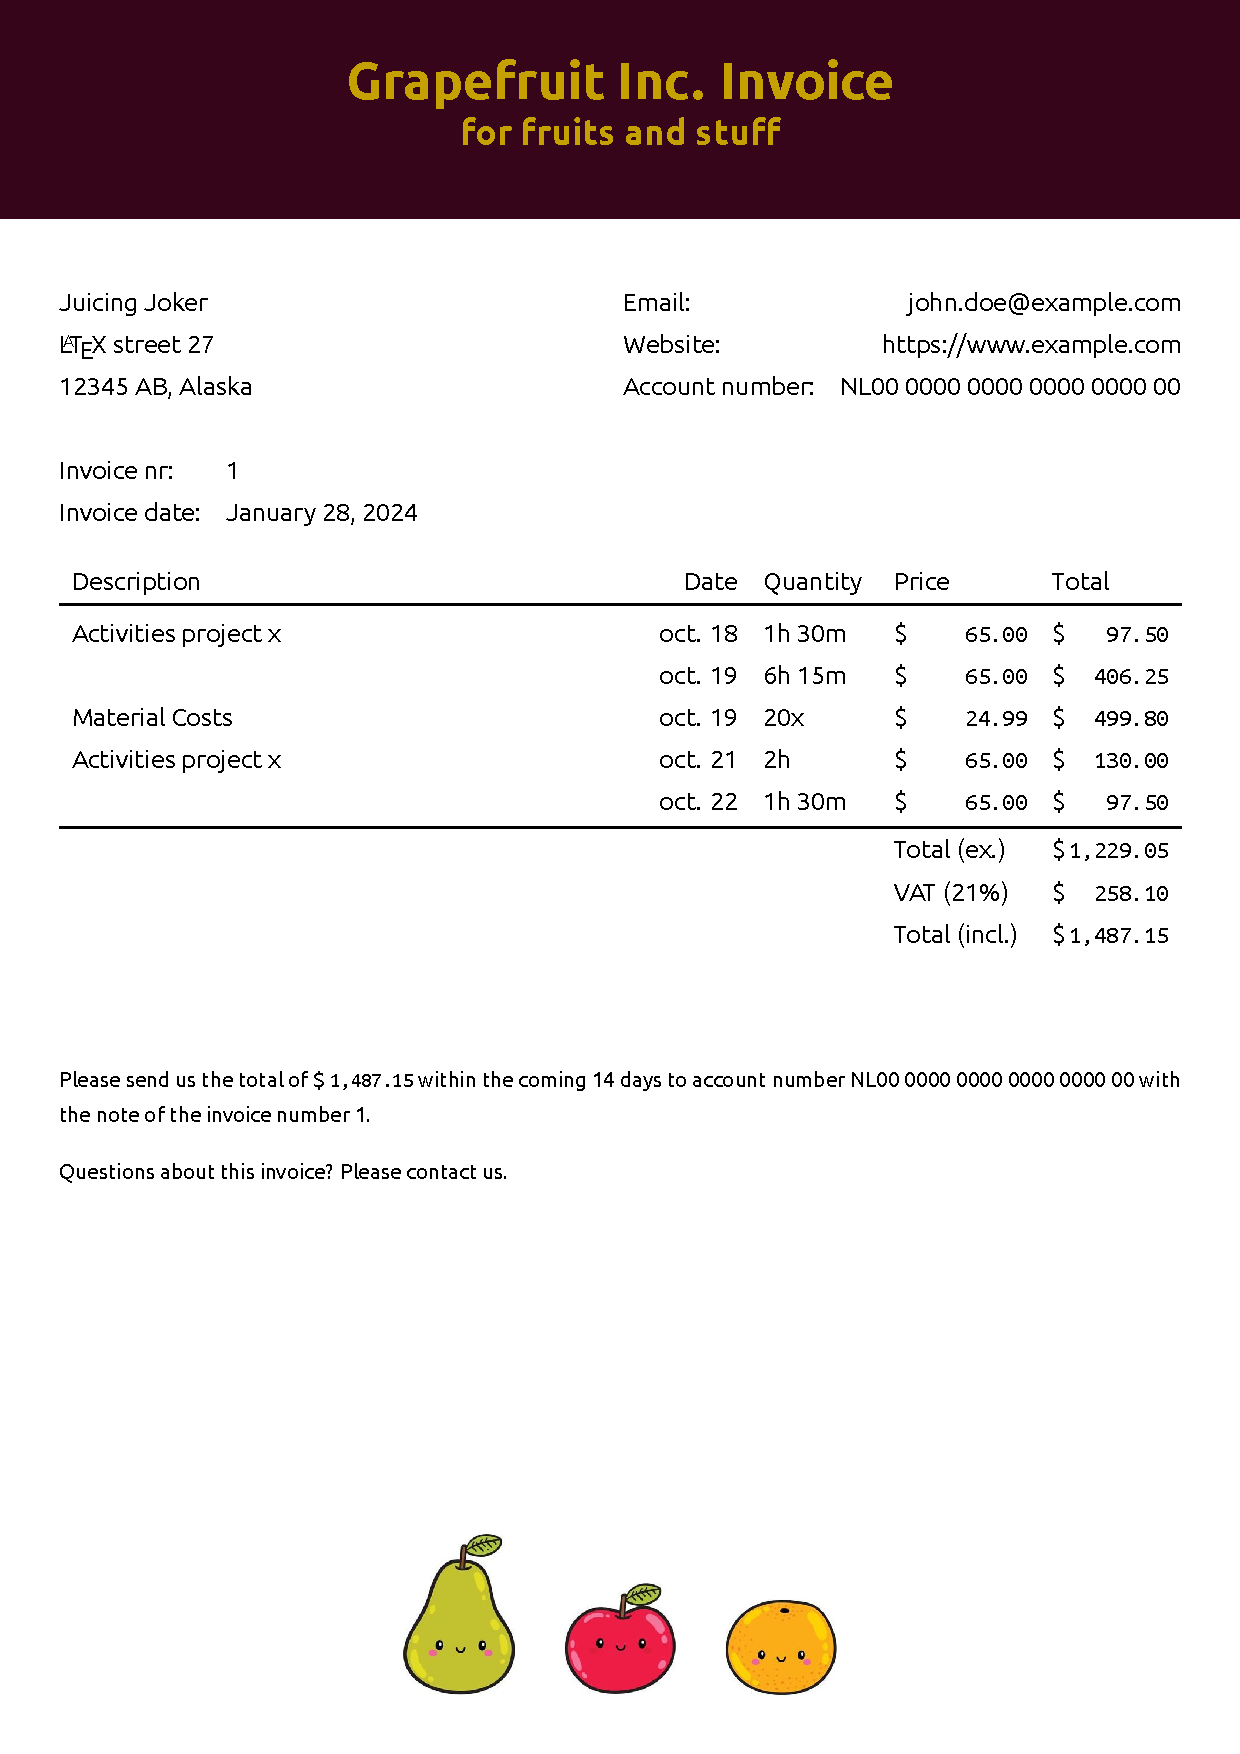
\includegraphics[width=\linewidth]{ginvoice/ginvoice.pdf}
    \caption{Voorbeeldfactuur gegenereerd door GinVoice}
    \label{fig:voorbeeldfactuur}
\end{figure}
Het bovenstaande voorbeeld toont een gegenereerde factuur met behulp van de huidige implementatie van GinVoice.
Echter, op dit moment vereist het genereren van dit voorbeeld Python, wat voor template makers die hoofdzakelijk \LaTeX\ gebruiken, ongewenst is.
In het volgende hoofdstuk zullen we deze situatie aanpakken en laten zien hoe dit voorbeeld rechtstreeks kan worden gegenereerd met \LuaLaTeX.
